\chapter{Introducción a la librería gráfica}
Una librería gráfica es una librería diseñada para ayudar a renderizar gráficos computados a un monitor. Esto típicamente involucra procurar de versiones optimizadas de funciones que llevan tareas de renderización comunes. Esto se puede hacer puramente con el software funcionando en la CPU, como es común en los sistemas enlazados o con hardware accelerado por una GPU, más común en los PCs. Utilizando estas funciones un programa puede ensablar una imagen para ser mostrada en un monitor. Eso le permite al programador saltarse el paso de crear y optimizar estas funciones, y le permite centrarse en construir el programa gráfico. Las librerías gráficas se usan principalmente en videojuegos y simulaciones.
Algunos ejemplos de librerías gráficas son los siguientes:
\begin{itemize}
\item{Direct3D}
\item{Mantle}
\item{Metal}
\item{OpenGL}
\item{Vulkan}
\end{itemize}
Para este proyecto se ha tomado como referencia OpenGL.

\newpage
\section{Pasos que sigue el motor gráfico}
Para mostrar en una pantalla 2D una escena 3D se siguen unos pasos conceptuales que se describirán a continuación: 
\subsection{Espacio local del objeto}
Es el espacio en el que se definen las coordenadas de los vértices, las normales y otros. Esto ocurre antes de que tome lugar cualquier transformación. Las coordenadas son relativas al centro del objeto en cuestión. 

Tomemos como ejemplo el siguiente cuadrado, éste tiene las siguientes coordenadas:
\[
E = (0, 3) \hspace*{0.5cm}
F = (0, 0) \hspace*{0.5cm} 
G = (3, 0) \hspace*{0.5cm} 
H = (3, 3) \hspace*{0.5cm} 
\]

\begin{figure} [h!]
  \centering
  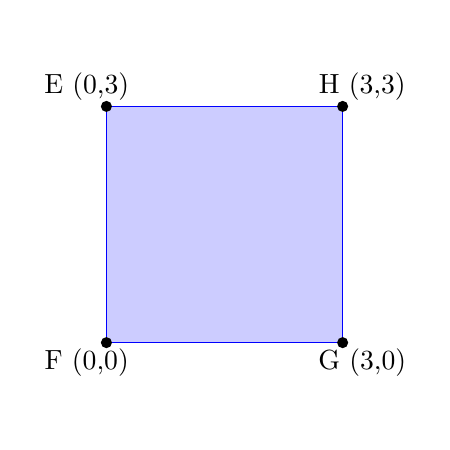
\begin{tikzpicture}
    \clip (0,0) rectangle (5,5);
    \draw [-,color=blue]
    (1,1) -- (4,1) -- (4,4) -- (1,4) -- (1,1);
    \fill [color=blue, opacity=0.2]
    (1,1) -- (4,1) -- (4,4) -- (1,4) -- (1,1);

    \draw
    (0.75,0.75) node {F (0,0)}
    (4.25,0.75) node {G (3,0)}
    (4.25,4.25) node {H (3,3)}
    (0.75,4.25) node {E (0,3)};

    \fill
    (1,1) circle (2pt)
    (4,1) circle (2pt)
    (4,4) circle (2pt)
    (1,4) circle (2pt);
    
  \end{tikzpicture}
  
\end{figure}

Ahora, los valores de estas coordenadas son transladados al espacio del mundo, y por lo tanto, los valores de las coordenadas cambiarán.
\newpage

\subsection{Espacio global}
Es el espacio en el que todos los objetos que hay en la escena están colocados en valores \textit{absolutos} relativos a un punto arbitario.

\begin{figure} [h!]
  \centering
  
\definecolor{qqqqff}{rgb}{0,0,1}\definecolor{rvwvcq}{rgb}{0.08235294117647059,0.396078431372549,0.7529411764705882}\definecolor{cqcqcq}{rgb}{0.7529411764705882,0.7529411764705882,0.7529411764705882}\begin{tikzpicture}[line cap=round,line join=round,>=triangle 45,x=1cm,y=1cm]\draw [color=cqcqcq,, xstep=1cm,ystep=1cm] (-0.8954391833090678,4) grid (8.899624154736587,8.625717670298478);\draw[->,color=black] (0,3.5) -- (0,8.5);\foreach \y in {4,5,6,7,8}\draw[shift={(0,\y)},color=black] (2pt,0pt) -- (-2pt,0pt) node[left] {\footnotesize $\y$};\clip(-0.8954391833090678,1.7979314035066118) rectangle (7,9);\fill[line width=1pt,color=qqqqff,fill=qqqqff,fill opacity=0.15] (3,5) -- (6,5) -- (6,8) -- (3,8) -- cycle;\draw [line width=0.5pt,color=qqqqff] (3,5)-- (6,5);\draw [line width=0.5pt,color=qqqqff] (6,5)-- (6,8);\draw [line width=0.5pt,color=qqqqff] (6,8)-- (3,8);\draw [line width=0.5pt,color=qqqqff] (3,8)-- (3,5);\begin{scriptsize}\draw [fill=black] (3,5) circle (2pt);\draw[color=black] (3.0858504808186202,5.239292743321078) node {$M (3,5)$};\draw [fill=black] (6,5) circle (2pt);\draw[color=black] (6.085452282558659,5.239292743321078) node {$N (6,5)$};\draw [fill=black] (6,8) circle (2pt);\draw[color=black] (6.085452282558659,8.238894545061104) node {$O (6,8)$};\draw [fill=black] (3,8) circle (2pt);\draw[color=black] (3.0858504808186202,8.238894545061104) node {$P (3, 8)$};\end{scriptsize}\end{tikzpicture}
  \caption{Todos los puntos del cubo se han desplazado 3 unidades en el eje X y 5 unidades en el eje Y con respecto a la figura anterior, una transformación ha ocurrido.}
  
  \end{figure}
  
\subsection{Espacio de vista}
En el espacio de vista se introduce una \textit{cámara} (coordenada desde la que se proyectará la imagen a mostrar)

\begin{minipage}{0.5\textwidth}
  \centering
    \definecolor{wrwrwr}{rgb}{0.3803921568627451,0.3803921568627451,0.3803921568627451}\definecolor{rvwvcq}{rgb}{0.08235294117647059,0.396078431372549,0.7529411764705882}\begin{tikzpicture}[thick,scale=0.6, every node/.style={scale=1}, line cap=round,line join=round,>=triangle 45,x=1cm,y=1cm]\clip(-8,-0.8073256135157997) rectangle (3.3936789799010794,10);\fill[line width=2pt,color=blue,fill=blue,fill opacity=0.10000000149011612] (-6,3) -- (-5,6) -- (-4,3) -- cycle;\fill[line width=2pt,color=blue,fill=blue,fill opacity=0.10000000149011612] (-5,6) -- (-4,4) -- (-4,3) -- cycle;\fill[line width=0.4pt,color=blue,fill=blue,fill opacity=0.1] (-3,7) -- (-3,5) -- (-1,5) -- (0,6) -- (0,8) -- (-2,8) -- cycle;\draw [line width=0.4pt,color=rvwvcq] (-6,3)-- (-5,6);\draw [line width=0.4pt,color=rvwvcq] (-4,3)-- (-6,3);\draw [line width=0.4pt,color=rvwvcq] (-5,6)-- (-4,4);\draw [line width=0.4pt,color=rvwvcq] (-4,4)-- (-4,3);\draw [line width=0.4pt,color=rvwvcq] (-4,3)-- (-5,6);\draw [line width=2pt,color=wrwrwr] (-7.8,1)-- (-2.2,12.4);\draw [line width=2pt,color=wrwrwr] (-7.8,1)-- (3.5,5.6);\draw (-7.561595933738325,1.0141538299567745) node[anchor=north west] {Cámara};\draw [line width=0.4pt,color=rvwvcq] (-3,7)-- (-2,8);\draw [line width=0.4pt,color=rvwvcq] (-3,7)-- (-3,5);\draw [line width=0.4pt,color=rvwvcq] (-3,5)-- (-1,5);\draw [line width=0.4pt,color=rvwvcq] (-1,5)-- (0,6);\draw [line width=0.4pt,color=rvwvcq] (0,6)-- (0,8);\draw [line width=0.4pt,color=rvwvcq] (0,8)-- (-2,8);\draw [line width=0.4pt,color=rvwvcq] (-2,8)-- (-3,7);\draw [line width=0.4pt,color=rvwvcq] (-3,7)-- (-1,7);\draw [line width=0.4pt,color=rvwvcq] (-1,5)-- (-1,7);\draw [line width=0.4pt,color=rvwvcq] (-1,7)-- (0,8);
    \end{tikzpicture}
\end{minipage}
\begin{minipage}{0.5\textwidth}
  \centering
  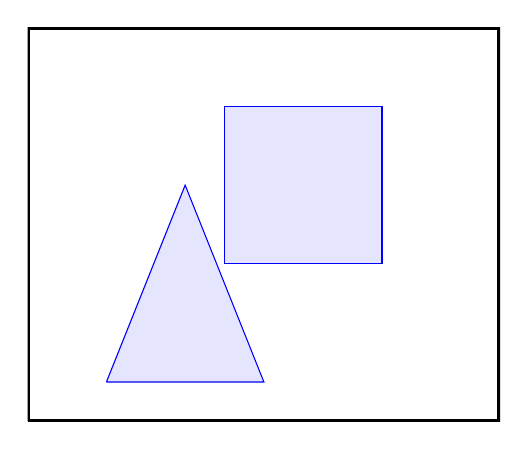
\begin{tikzpicture}
    \clip (0,0) rectangle (6,5)
    (1,0.5) node (1) {}
    (2,  3) node (2) {}
    (3,0.5) node (3) {}
    (2.5,2) node (4) {}
    (4.5,2) node (5) {}
    (4.5,4) node (6) {}
    (2.5,4) node (7) {};
    
    \draw[-, color=blue]
    (1.center) -- (2.center) -- (3.center) -- (1.center);
    
    \draw[-, color=blue]
    (4.center) -- (5.center) -- (6.center) -- (7.center) -- (4.center);

    \fill[color=blue, opacity=0.1]
    (1.center) -- (2.center) -- (3.center) -- (1.center)
    (4.center) -- (5.center) -- (6.center) -- (7.center) -- (4.center);

    \draw[-, line width=2pt, color=black]
    (0,0) -- (6,0) -- (6,5) -- (0,5) -- (0,0);
    
  \end{tikzpicture}
\end{minipage}
\newpage

\subsection{Espacio de clipping y división de perspectiva}
En este espacio, la escena se inserta en un cubo de coordenadas opuestas (-1,-1,-1) a (1,1,1) y se recortan los objetos que sobresalen.

\subsection{Espacio de la pantalla}
Consiste en mapear las coordenadas NDC a la ventana. $X$ y $Y$ son íntegros, relativos a la esquina izquierda inferior de la ventana. Las $Z$ son escaladas y sesgadas a [0,1]. La rasterización se produce en este espacio.
